\chapter{Alcances de la Memoria}
\label{alcansces}

\section{Problema a resolver}

Actualmente Chile no cuenta con plantas de energía solar fotovoltaica conectadas a sus redes centrales de distribucion (SIC\gloss{SIC}, SING\gloss{SING}, SM\gloss{SM}, SA\gloss{SA}), debido a problemas legales y de normativas tecnicas, la mayoria de las plantas solares que generan energia en chile son plantas aisladas o conectadas a sistemas de distribucion privados, como por ejemplo Calama Solar 3\cite{plantaSolar:1}, Subsole\cite{subsole:2,} entre otras.

La Red Solar para Latinoamerica y el Caribe(RedSolLac) tiene por objetivo contribuir al desarrollo y aprovechamiento de la energia solar fotovoltaica. Ello mediante una plataforma de difusión de información, que facilita la cooperación y colaboración mutua de instituciones, empresas, profesionales y personas interesadas.
Para apoyar la construccion de de la plataforma de difucion de RedSolLac, Esta ha encargado el desarrollo de una aplicacion infromatica, que permita exponer de forma grafica informacion de produccion de energia para plantas solares fotovoltaicas, asi como de estaciones de monitoreo meteorologicas, ademas requiere la construccion de una herramienta que le permita calcular costos de construccion y produccion de energia para apoyar en la toma de desiciones respecto de la construccion de nuevas plantas de energia solar.

\begin{figure}[h!]
        \centering
        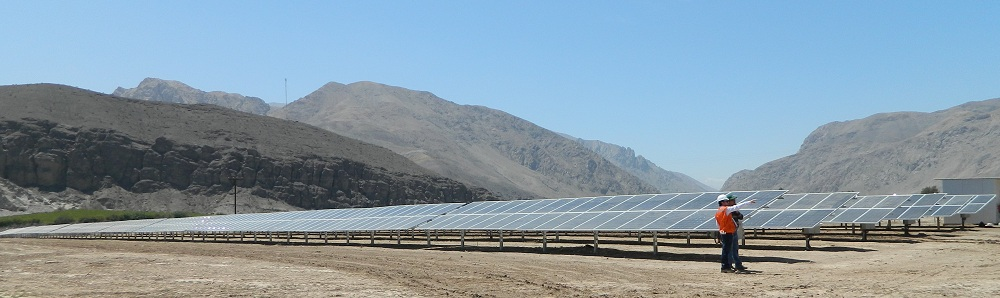
\includegraphics[scale=1.5]{images/plantaSubSoleLorosAmarilla}
        \caption{Planta fotovoltaica 307,2 kWp, sector Los Loros - Tierra Amarilla, región de Atacama - Chile}
\end{figure}
\begin{figure}[h!]
        \centering
        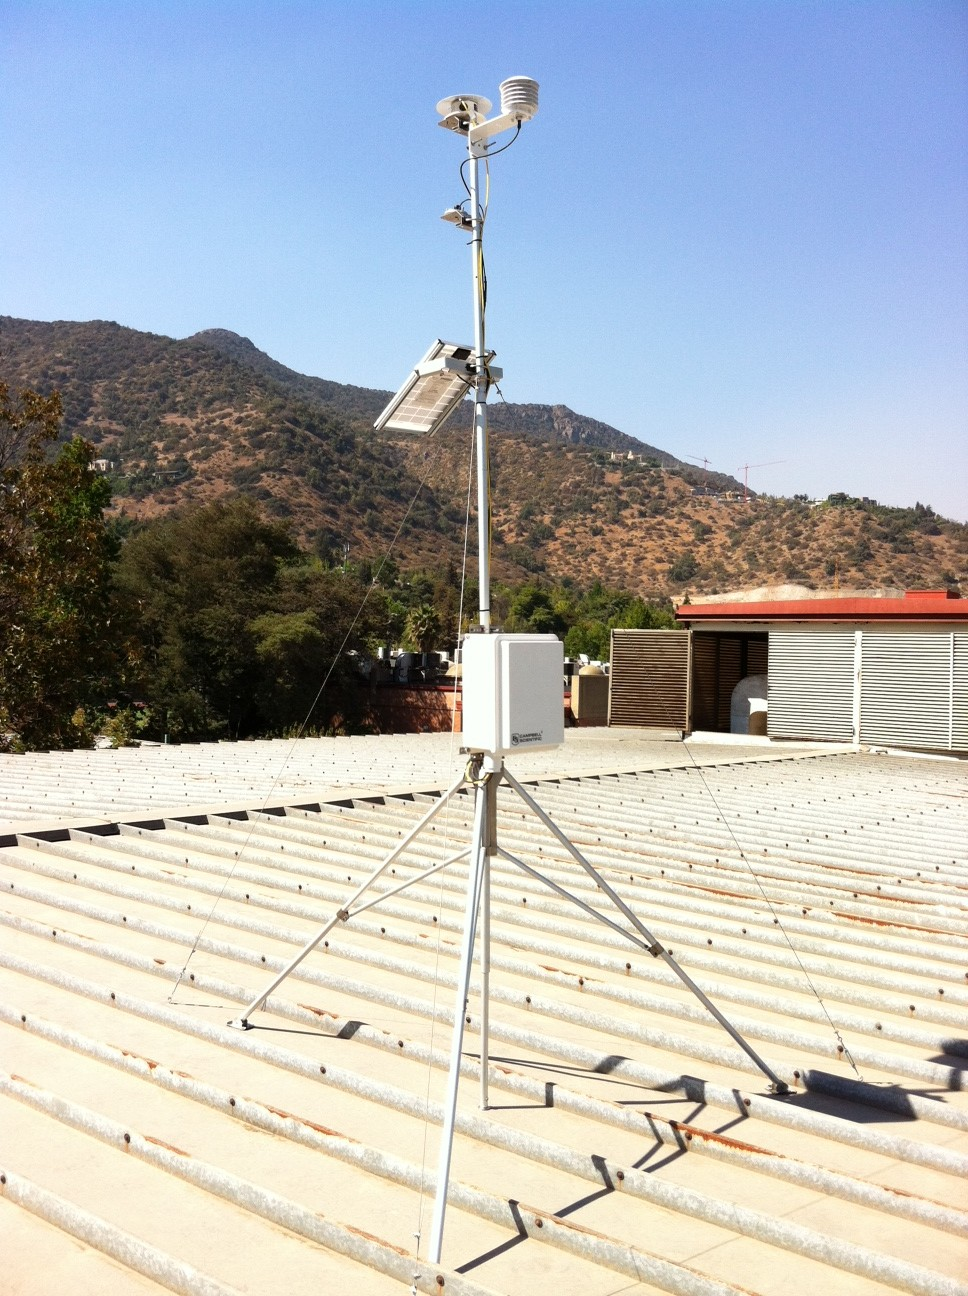
\includegraphics[scale=0.1]{images/estacionMedicionFch}
        \caption{Estación de medición de radiación solar en Fundación Chile, Vitacura - Santiago.}
\end{figure}

Para el desarrollo de este sistema Fundacion Chile utilizara datos de produccion de energia provenientes de diferentes fuentes, entre ellas la nueva planta de Subsole(Fig 2.1), datos de adquisicion propia mediante una estacion meteorologica ubicada en la comuna de Vitacura en la Región Metropolitana(Fig. 2.2) y datos estadisticos publicados por diferentes entidades referentes del tema\cite{datosSolares:1}.

Subsole S.A\cite{subsole:1} es una empresa exportadora de frutas a nivel nacional, a finales del año 2011 finalizo la construccion de una planta solar de 307 kWp\cite{subsole:2} con el objetivo de subministrar corriente elctrica al proceso de riego para la produccion de frutas en el valle de Copiapo en la III Region de Atacama. La planta solar de Subsole es un proyecto pionero para el bombeo de agua mediante el uso de la energía solar para una empresa exportadora de frutas y pretende ser un proyecto modelo para el desarrollo de las ERNC\gloss{ERNC} en los proximos años.\\

El sistema informático actual recibe datos de los inversores y su sistema de medición de energía y almacenamiento de datos, los envía a un sistema privado, el cual no permite la publicación y uso de información, por lo que es necesario implementar un sistema que permita publicar dicha información.\\

\begin{figure}[h!]
        \centering
        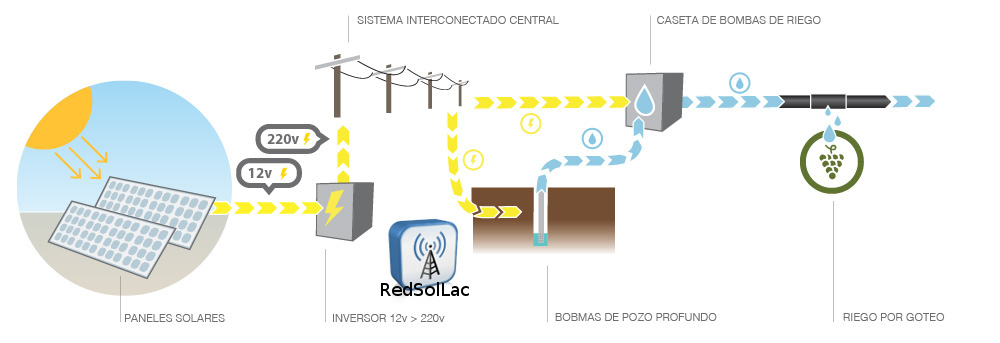
\includegraphics[scale=0.4]{images/plantaSubSoleEsquema}
        \caption{Esquema planta fotovoltaica Subsole 307,2 kWp(STC) a la red eléctrica EMELAT - Región de Atacama}
\end{figure}

La planta eléctrica de Subsole(Fig. 2.3), tiene como objetivo producir suficiente energía que le permita alimentar los motores que extraen el agua de los pozos destinados al riego por goteo. El proyecto original se diseño con la intencion de vender la energia al SIC y que el sistema de riego utilizara al mismo tiempo energia del SIC, actuando la planta como un productor de energia que le permitiria vender o comprar energia dependiendo de la produccion o demanda de esta. Sin embargo esto no se ha podido conretar por dificultades legales, mientras tanto la energia que produce la planta va dirigida directamente al sistema electrico interno.
Los inversores que figuran en el esquema permiten convertir la electricidad producida por los paneles a corriente alterna y 220 Volt, adicionalmente los inversores tienen la capacidad de registrar la información de potencia que pasa por ellos. Dentro del trabajo realizado en esta memoria se contempla instalar un sistema de comunicación para los inversores que permita enviar la información directamente a una base de datos de la RedSolLac en Internet.\\

Ademas se cuenta con una estación de medición de radiación solar, temperatura y humedad ambiente, instalada en Fundación Chile, en la comuna de Vitacura, Santiago de Chile. Esta estacion(Fig. 2.2) en conjunto con la estación meteorológica de la planta fotovoltaica(Fig. 2.3), proporcionarán la información de radiación solar para la calculadora fotovoltaica. Se espera en el futuro incorporar más estaciones de medición.\\

Los principales actores y usuarios de este sistema son todos los miembros de la RedSolLAC, interesados en recibir y compartir información relacionada con la energía solar fotovoltaica. En todo caso la plataforma es abierta por lo que cualquier otro usuario puede acceder a esta información.\\

El BID a través del proyecto RedSolLac que desarrolla la Fundación Chile espera conectar a los actores claves en el desarrollo de la energia solar fotovoltaica de Latinoamérica y el Caribe. En la actualidad, existen pocos actores en la región, por lo que el conocimiento técnico en esta materia se reduce a experiencias de universidades y algunas iniciativas privadas aisladas. La información generada por la planta fotovoltaica Subsole busca convertirse en un sitio de referencia para el estudio y desarrollo de nuevas iniciativas solares.\\

El desarrollo de esta memoria permite la comunidad de la RedSolLac contar con una gran base de datos para ofrecer a todos sus usuarios, así como diversas aplicaciones en su plataforma para la difunción y el patrocinio de la energía solar en la región. Una red como esta potencia el desarrollo de todas las energías renovables no convencionales(ERNC) especialmente la solar fotovoltaica, esto se traduce en un beneficio medioambiental directo para toda la comunidad tanto pertenecientes a la red como a la población en general.

\section{Objetivo principal de la solución}
Desarrollar e implementar un sistema informático para la RedSolLAC que permita interconectar equipos y estaciones de medición solar para la recolección y explotación de datos e información técnica provenientes de una planta solar ubicada en la región de Atacama, Chile.

\section{Objetivos específicos de la solución}
\begin{itemize}
\item Interconectar los diferentes sistemas que componen las estaciones de medición para que exista una comunicación efectiva entre dichos sistemas y una base de datos común en Internet.
\item Desarrollo de un sistema Web capaz de procesar y publicar la información recopilada de una planta de energía solar de gran potencia, ubicada en la región de Atacama.
\item Desarrollo de una calculadora online para sistemas fotovoltaicos, que permita dimensionar y estimar los costos de produccion de energia electrica.
\item Realizar pruebas de la plataforma en conjunto con todos sus componentes, comparar los datos obtenidos con datos recopilados de otras fuentes. Estas prubas permitiran validar el funcionamiento del software asi como la acertividad del metodo de calculo y estimacion electrica implementado en la solución.
\end{itemize}

\section{Requerimientos de software}

graficar cuervas en base a los datos obtenido por la estacion
el grafico debe poder escalarse
selecionar opcion para el periodo de tiempo a graficar
agregar o quitar curvas en la grafica
los parametros de la grafica debe ser entendible y legible por cualquier elctor
la estacion debe conectarse a internet y registrar datos cada 1 minutoen una base de datos externa
la estacion debe tener un respaldo de los datos en caso de perder conexion a internet
debe existir un procedimiento de respaldo de datos y restauracion en casos de eventos
el software debe tener una interfaz que permita la descarga de datos de acuerod a un rango de fechas dado por el usuario
debe proporcionar un modulo que muestre las ultimas mediciones obtenidas con la posibilidad de ser integradas en un sitio web
debe poder integrarse con worpress
posibilidad de configurar o conectar diferentes estaciones
mostrar las caracteristicas de la estacion que grafica
las curvas deben tener colores diferentes
los datos deben ser obtenidos asincronicamente de acuerdo a los periodos de tiempo
la generacion de la grafica no debe demorar mas de 3 segundos


implementar modelo de calculo para la radiacion que admita multiples variables del medio que influye el resultado
mostrar una tabla resumen con datos y costos de produccion de energia mensual y anual
permitir escoger angulo de orientacion e inclinacion del los modulos
ingreso del factor de eficiencia de la instalacion
permitir que el usuario ingrese parametros de ubicacion ....  

\begin{figure}[h!]
        \centering
        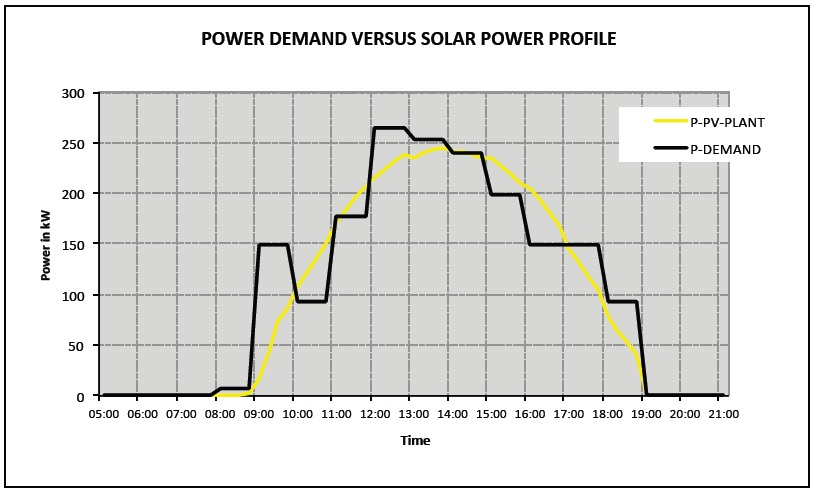
\includegraphics[scale=0.5]{images/demandaGeneracionSubSole}
        \caption{\tiny Gráfico de ejemplo de la curva de demanda de energía versus la generación de energía solar fotovoltaica en la planta Subsole.}
\end{figure}
